\section{Exercise 6.2 Illustrate global sensitivity analysis}
\textbf{Problem:} Using {\tt AMPL}, make an original example, with at least three constraints, graphing the objective value of $(P)$, as a single {\tt b[i]} is varied from $-\infty$ to $+\infty$. As you work on this, bear in mind Theorem 6.3.

\textbf{Solution:} Consider the standard-form problem (P) with $m=3$ and $n=5$

\[
\tag{P}
\begin{array}{rrcl}
 \min & c'x  &      &   \\
      &  Ax  &   =  & b~; \\
      &   x  & \geq & \mathbf{0}~,
\end{array}
\]

where
\[
\begin{array}{ccc}
A  :=  \left(
  \begin{array}{ccccc}
    1 & -1 & 0 & -1 & 0  \\
    0 & -4 & 2 & 2 & 0 \\
    0 & -9 & 0 & 6 & 3\\
  \end{array}
\right)~, &
b  :=  (1,2,18)'~,&
c  :=  (16, 7, 20, 10, 4)'~.\\

\end{array}
\]

Using {\tt AMPL}, at each time we vary only one $b_i$ from $b$ and check the range of $b_i$ in which the optimal basis for (P) keeps the same. We show the optimal basis as follows:

\begin{table*}[!h]
\centering
\small
\begin{tabular}{|c|c|c|c|}\hline

$b_1$ & $(-\infty, -13)$ & $(-13, -1)$ & $(-1,+\infty)$ \\\hline
optimal basis $\beta$ & $\{2,3,4\}$ & $\{2,4,5\}$ & $\{1,4,5\}$ \\\hline
$c'_{\beta}A^{-1}_{\beta}$ & $(-12.8~~10~~-3.8)$ & $(-23/3~~-17/6~~4/3)$ & $(16~~9~~4/3)$ \\\hline
objective value & $-12.8b_1-48.4$& $(-23/3)b_1+55/3$ & $16b_1+42$ \\\hline 

\end{tabular}
\\
\begin{tabular}{|c|c|c|c|}\hline

$b_2$ & $(-\infty, 0)$ & $(0, 6)$ & $(6,+\infty)$ \\\hline
optimal basis $\beta$ & $\{1,2,5\}$ & $\{1,4,5\}$ & $\{1,3,4\}$ \\\hline
$c'_{\beta}A^{-1}_{\beta}$ & $(16~~-8.75~~4/3)$ & $(16~~9~~4/3)$ & $(16~~10~~18)$ \\\hline
objective value & $-8.75b_2+40$& $9b_2+40$ & $10b_2+34$ \\\hline 

\end{tabular}
\\
\begin{tabular}{|c|c|c|c|}\hline

$b_3$ & $(-\infty, 0)$ & $(0, 6)$ & $(6,+\infty)$ \\\hline
optimal basis $\beta$ & $\{1,2,3\}$ & $\{1,3,4\}$ & $\{1,4,5\}$ \\\hline
$c'_{\beta}A^{-1}_{\beta}$ & $(16~~10~~-7)$ & $(16~~10~~1)$ & $(16~~9~~4/3)$ \\\hline
objective value & $-7b_3+36$& $b_3+36$ & $(4/3)b_3+34$ \\\hline 

\end{tabular}
\caption{Changing single $b_i$ from $-\infty$ to $+\infty$}
\label{tab:p2}
\end{table*}

As we get the above data from {\tt AMPL}, we graph the objective value of (P) as a single $b_i$ is varied from $-\infty$ to $+\infty$ in Figure \ref{fig:p2}.

\begin{figure}[h!!]
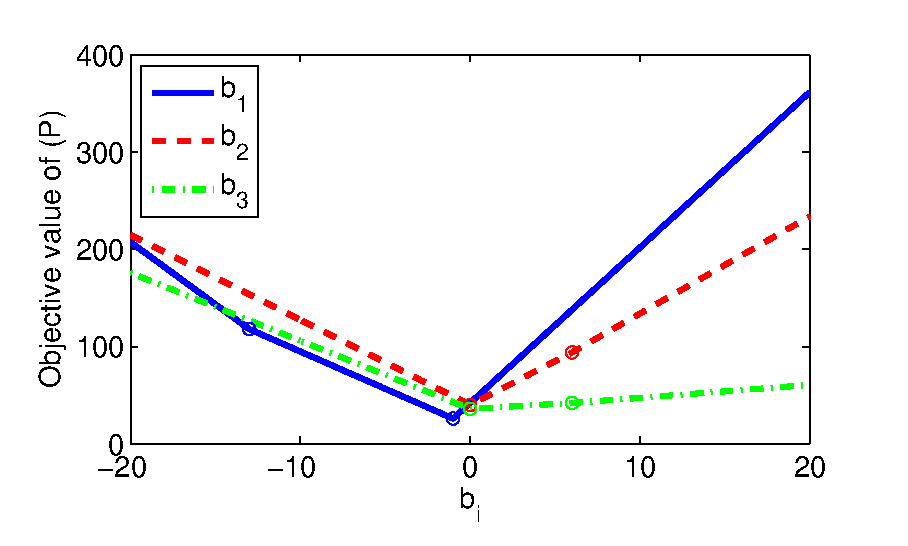
\includegraphics[width=0.7\textwidth]{p2/p2.eps}
\caption{Objective value of (P) as a single $b_i$ is varied from $-\infty$ to $+\infty$}\label{fig:p2}
\end{figure}